\chapter{Théorie des Circuits}

Dans ce chapitre, nous réitérons plusieurs éléments de la théorie des circuits élémentaires qui sont nécessaires pour comprendre les circuits électroniques de base. Ces éléments comprennent des composants passifs tels que les résistances, les condensateurs et les bobines, les lois de Kirchhoff, la représentation de phasor et l'impédance complexe, ainsi que plusieurs transformations de circuit pour faciliter l'analyse.

\section{Composants Passifs}
Dans les circuits électroniques que nous étudierons, nous rencontrons quatre types d'éléments:
\begin{itemize}
	\item Sources : ce sont des systèmes relativement complexes avec deux bornes qui fournissent soit une tension, soit un courant. Les sources peuvent être constantes, c'est-à-dire que le courant ou la tension générée ne varie pas avec le temps, ou elles peuvent générer un courant ou une tension qui varie dans le temps. Dans le premier cas, nous les appelons sources de courant continu (DC), dans le second cas, nous parlons de sources de courant alternatif (AC), généralement avec une valeur moyenne de zéro.
	\item Éléments linéaires : ceux-ci peuvent être passifs, tels que les résistances, les condensateurs ou les bobines, ou actifs, tels que les sources de courant ou de tension dépendantes. Ces dernières sont des sources qui dépendent linéairement d'autres courants ou tensions dans le circuit.
	\item Éléments non linéaires, tels que les diodes et les transistors. L'étude de l'électronique concerne ces éléments et la façon dont ils sont utilisés dans les circuits.
	\item Conducteurs, qui connectent les différents éléments discrets. Nous supposons qu'ils sont idéaux : ils n'ont pas de résistance, d'inductance ou de capacité. Si l'un de ces défauts est présent dans des conducteurs réels, ils seront modélisés comme des éléments discrets séparés.
\end{itemize}
Nous utilisons toujours l'approximation quasi-statique, où la valeur du courant dans une branche est la même partout dans cette branche. Ceci est valable lorsque les dimensions du circuit sont beaucoup plus petites que la longueur d'onde du signal.



The most important linear passive components are:
\begin{itemize}
	\item A \emph{resistor} is an element that resists the flow of current due to an applied voltage. The current-voltage relation is:
	$$v_R = R\;i_R$$
	The resistance of a resistor is measured in ohms ($\Omega$).
	\item A \emph{capacitor} is a passive electronic component that stores electrical energy in an electric field. It consists of two conductive plates separated by an insulating material, called the dielectric.\\
	When a voltage is applied across the plates of a capacitor, electrical charge $Q$ accumulates on the plates, creating an electric field between them.
	The current-voltage relation is
	$$v_C  = \frac{Q}{C} = \frac{1}{C} \int i_C \; dt$$
	or 
	$$i_C = C  \; \frac{dv_C}{dt}$$
	A capacitor resists a sudden change in voltage across its terminals. The capacitance of a capacitor is measured in farad ($F$).
	\item An \emph{inductor} is a passive electronic component that stores electrical energy in a magnetic field. It consists of a coil of wire, often wrapped around a core made of a magnetic material, such as iron or ferrite.\\	
	When an electric current flows through an inductor, a magnetic field is created around the coil. The strength of the magnetic field is proportional to the amount of current flowing through the coil. When the current changes, the magnetic field changes, inducing a voltage across the coil that opposes the change in current. Thus, an inductor resists a sudden change in current.
	The current-voltage relation is
	$$
	v_L = L  \;  \frac{di_L}{dt}
	$$
	or also
	$$
	i_L = \frac{1}{L}\int v_L  \;  dt
	$$
	The inductance of an inductor is measured in henry ($H$).
	
\end{itemize}

\begin{figure}[h!]
	\centering
	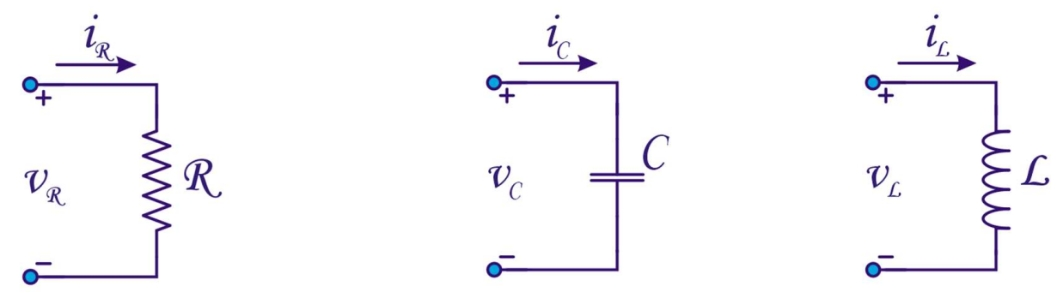
\includegraphics[width=14cm]{figures/ch00/passive.jpg}
	\caption{Resistor (left), capacitor (middle) and inductor (right)}
	\label{fig:passive}
\end{figure}


Les composants passifs linéaires les plus importants sont :
\begin{itemize}
	\item Une \emph{résistance} est un élément qui résiste à l'écoulement du courant en raison d'une tension appliquée. La relation courant-tension est :
	$$v_R = R\;i_R$$
	
	La résistance d'une résistance est mesurée en ohms ($\Omega$).
	\item Un \emph{condensateur} est un composant électronique passif qui stocke de l'énergie électrique dans un champ électrique. Il se compose de deux plaques conductrices séparées par un matériau isolant appelé diélectrique.\\
	Lorsqu'une tension est appliquée aux plaques d'un condensateur, une charge électrique $Q$ s'accumule sur les plaques, créant un champ électrique entre elles.
	
	La relation courant-tension est
	$$v_C  = \frac{Q}{C} = \frac{1}{C} \int i_C \; dt$$
	ou encore 
	$$i_C = C  \; \frac{dv_C}{dt}$$
	
	Un condensateur résiste à un changement soudain de tension à ses bornes. La capacité d'un condensateur est mesurée en farads ($F$).
	\item Une \emph{inductance} est un composant électronique passif qui stocke de l'énergie électrique dans un champ magnétique. Elle se compose d'une bobine de fil, souvent enroulée autour d'un noyau en un matériau magnétique tel que le fer ou la ferrite.\
	Lorsqu'un courant électrique circule dans une inductance, un champ magnétique est créé autour de la bobine. La force du champ magnétique est proportionnelle à la quantité de courant circulant dans la bobine. Lorsque le courant change, le champ magnétique change, ce qui induit une tension à travers la bobine qui s'oppose au changement de courant. Ainsi, une inductance résiste à un changement soudain de courant.
	La relation courant-tension est
	$$
	v_L = L  \;  \frac{di_L}{dt}
	$$
	ou encore
	$$
	i_L = \frac{1}{L}\int v_L  \;  dt
	$$
	L'inductance d'une inductance est mesurée en henry ($H$).
	
\end{itemize}

\begin{figure}[h!]
	\centering
	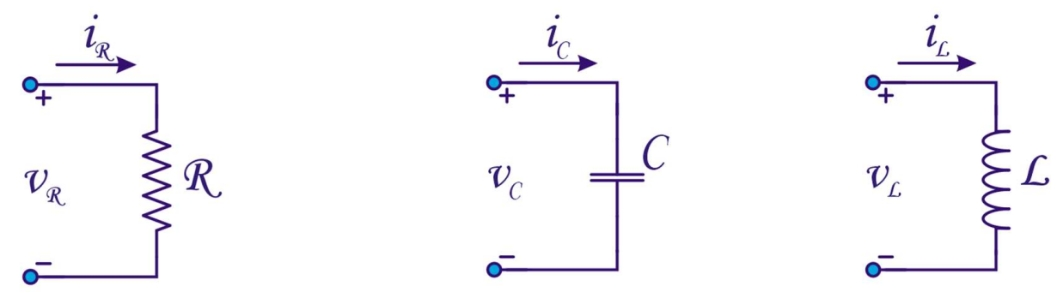
\includegraphics[width=14cm]{figures/ch00/passive.jpg}
	\caption{Résistance (à gauche), condensateur (au milieu) et inductance (à droite)}
	\label{fig:passive}
\end{figure}

\section{Lois de Kirchhoff}
\subsection{Loi des tensions de Kirchhoff}
La loi des tensions de Kirchhoff (LTV) stipule que la somme des différences de potentiel (tensions) autour d'une boucle fermée est nulle :
\begin{equation}
	\sum_{k=1}^n v_k = 0
	\label{eq:KVL}
\end{equation}
La LTV est en réalité une reformulation de la loi de Faraday $\nabla \times \vec{E} = -\frac{\partial B}{\partial t} = 0$, où l'on suppose que les champs magnétiques (variables dans le temps) sont confinés à chaque composant et que le champ dans la région extérieure au circuit est négligeable.

\begin{minipage}{.5\textwidth}
	\centering
	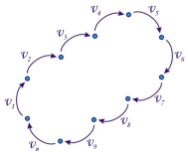
\includegraphics[width=5cm]{figures/ch00/kvl.jpg}
	\captionof{figure}{Loi des tensions de Kirchhoff}
	\label{fig:kvl}
\end{minipage}
\begin{minipage}{.5\textwidth}
	\centering
	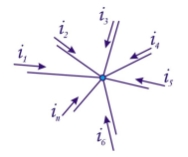
\includegraphics[width=5cm]{figures/ch00/kcl.jpg}
	\captionof{figure}{Loi des courants de Kirchhoff}
	\label{fig:kcl}
\end{minipage}%

\subsection{Loi des courants de Kirchhoff}
La loi des courants de Kirchhoff (LCK) affirme que dans un nœud d'un circuit électrique, la somme algébrique des courants est nulle :
\begin{equation}
	\sum_{k=1}^n i_k = 0
	\label{eq:KCL}
\end{equation}
ou de manière équivalente, que la somme des courants entrant dans ce nœud est égale à la somme des courants en sortant. La loi repose sur le fait qu'il n'y a pas d'accumulation de charges dans aucun nœud du réseau.

\subsection{Exemple}

Considérons le circuit de la figure \ref{fig:example1}. Avec KVL, on peut écrire :
$$
v_{in} = v_R + v_C = R \; i + v_C
$$
avec $i = C ; \frac{dv_C}{dt}$. L'équation pour trouver $v_C$ devient :
$$
v_{in} = RC \; \frac{dv_C}{dt} + v_C
$$
Si $v_{in}$ est soudainement allumé (par exemple, en fermant un interrupteur à $t=0$), alors $v_{in} = V_0 ; u(t)$ avec $u(t)$ la fonction échelon. On peut alors résoudre pour $v_C(t)$ :
\begin{align*}
	RC ; \frac{dv_C}{dt} + v_C &= V_0 \\
	\frac{dv_C}{dt} &= \frac{1}{RC} (V_0 - v_C) \\
	\frac{dv_C}{V_0 - v_C} &= \frac{dt}{RC} \\
	\int_0^{v_C} \frac{dv_C}{V_0 - v_C} &= \int_0^t \frac{dt}{RC} \\
	- \ln(V_0 - v_C) &= \frac{t}{RC} + K' \\
	v_C(t) &= V_0 - K e^{\frac{-t}{RC}}
\end{align*}
avec $K = V_0$ de telle sorte que $v_C(t=0) = 0$ :
$$
v_C(t) = V_0(1 - e^{\frac{-t}{RC}}) = V_0(1 - e^{-\frac{t}{T}})
$$

\begin{minipage}{.5\textwidth}
	\centering
	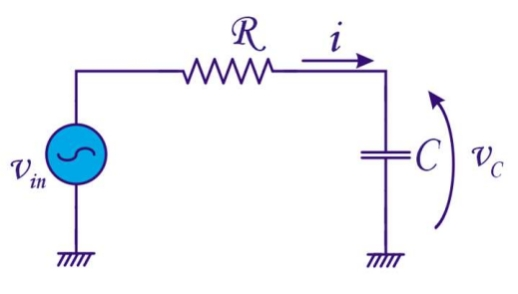
\includegraphics[width=6cm]{figures/ch00/example1.jpg}
	\captionof{figure}{}
	\label{fig:example1}
\end{minipage}
\begin{minipage}{.5\textwidth}
	\centering
	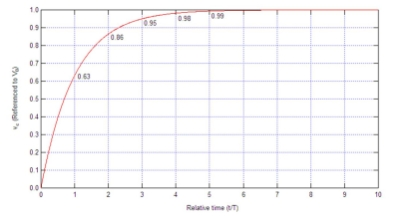
\includegraphics[width=9cm]{figures/ch00/first_order.jpg}
	\captionof{figure}{}
	\label{fig:first_order}
\end{minipage}%
\\Cette fonction est représentée dans la figure \ref{fig:first_order}. La tension $v_C$ augmente comme la réponse à un échelon d'un système du premier ordre, et atteint $63\%$ de la valeur finale après un temps caractéristique $T = RC$. Il faut $5T$ pour atteindre $99\%$ de la valeur finale.
\section{Représentation en fréquence}
\subsection{La transformation de Steinmetz}
Supposons qu'un signal sinusoïdal avec une fréquence $f = \omega/2\pi$ soit appliqué à un circuit ne contenant que des éléments linéaires. La théorie des systèmes linéaires nous enseigne alors que chaque courant et tension sera également une sinusoïde avec la même fréquence. Supposons que le courant dans un élément peut être écrit comme $I = I_0 \cos(\omega ; t) = Re{I_0 e^{j\omega t}}$. Dans ce cas, nous pouvons écrire :
\begin{itemize}
	\item Pour une résistance : $V_R = R ; I_R$
	\item Pour un condensateur : $V_C = \frac{1}{C} \int I_L \; dt = \frac{1}{C} \int I_0 e^{j\omega t} \; dt = \frac{1}{j\omega C} I_0 e^{j\omega t} = \frac{1}{j\omega C} \; I_C$
	\item Pour une inductance : $V_L = L \frac{dI_L}{dt} = L \frac{d(I_0 e^{j\omega t})}{dt} = j \omega L \; I_0 e^{j\omega t} = j \omega L \; I_L$
\end{itemize}
Ces relations sont la représentation en phaseur d'un signal sinusoïdal, ou les transformations de Steinmetz. Elles sont résumées dans la figure \ref{fig:steinmetz}.

\begin{figure}[h!]
	\centering
	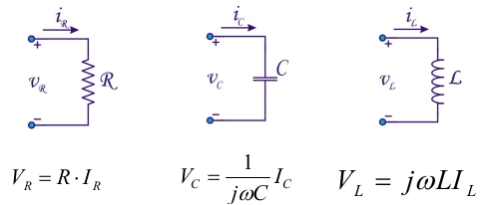
\includegraphics[width=10cm]{figures/ch00/steinmetz.jpg}
	\caption{}
	\label{fig:steinmetz}
\end{figure}

De cela, nous concluons que pour chaque élément, nous pouvons écrire:
$$
V = Z \cdot I
$$
où $Z$ est l'\emph{impédance complexe} de l'élément : $R$ pour une résistance, $\frac{1}{j\omega C}$ pour un condensateur et $j\omega L$ pour une bobine.\
Nous définissons également d'autres paramètres de circuit : $Y = \frac{1}{Z}$ comme l'\emph{admittance} telle que $I = Y \cdot V$, et $G = \frac{1}{R}$ comme la \emph{conductance} (mesurée en siemens ou A/V).

\subsection{La transformation de Laplace}
\label{sec:laplace}

La représentation phasorique ou la transformée de Steinmetz n'est possible que pour des signaux sinusoïdaux. Cette condition est parfois trop restrictive et nous avons besoin d'autres méthodes d'analyse. L'une de ces méthodes, qui est valable pour des signaux arbitraires $x(t)$, est la transformée de Laplace (unilatérale) $X(s)$, définie comme :
$$
\mathcal{L}[x(t)] = X(s) = \int_{t = 0}^{+\infty} e^{-st} x(t) dt
$$
avec $s$ la variable de Laplace complexe : $s = \sigma + j\omega$. Comme exemple, calculons $\mathcal{L}[\frac{dx(t)}{dt}]$ :
\begin{align*}
	\mathcal{L}[\frac{dx(t)}{dt}] &= \int_{t = 0}^{+\infty} e^{-st} \frac{dx}{dt} dt \\
	&= e^{-st} x(t) |_{t = 0}^{+\infty} - \int_{t = -\infty}^{+\infty} x(t) \frac{d(e^{-st})}{dt} dt \\
	&= \int_{t = 0}^{+\infty} s \; x(t) e^{-st} dt - x(0^+)\\
	&= s X(s) - x(0^+)
\end{align*}
Lorsque nous supposons que $x(0^+) = 0$, nous trouvons que $\mathcal{L}[\frac{dx(t)}{dt}] = s X(s)$. Un système linéaire avec une entrée $x(t)$ et une sortie $y(t)$ peut être décrit par une équation différentielle linéaire d'ordre supérieur :
\begin{align*}
	y(t) &= a_0 x(t) + a_1 \frac{dx}{dt} + a_2 \frac{d^2 x}{dt^2} + \ldots + b_1 \frac{dy}{dt} + b_2 \frac{d^2 y}{dt^2} + \ldots \\
	\Rightarrow \frac{Y(s)}{X(s)} &= \frac{a_0 + a_1 s + a_2 s^2 + \ldots}{1 - b_1 s - b_2 s^2 - \ldots}
\end{align*}
Ainsi, la transformée de Laplace de tout système linéaire peut être écrite comme le rapport de deux polynômes en $s$. Supposons que nous avons un système du premier ordre :
\begin{align}
	\frac{dy}{dt} &= \alpha \; y(t) + \beta \; x(t)
	\label{eq:first_order}
\end{align}
Si il n'y avait pas d'entrée $x(t)$, la solution serait :
$$
y(t) = C e^{\alpha t}
$$
Cette sortie reste finie pour $t \rightarrow \infty$ uniquement lorsque $\alpha \le 0$. C'est le critère de stabilité pour un système du premier ordre.\
Si nous prenons la transformée de Laplace de l'équation \ref{eq:first_order}, nous trouvons :
\begin{align*}
	s Y(s) &= \alpha ; Y(s) + \beta ; X(s) \\
	\Rightarrow \frac{Y(s)}{X(s)} &= \frac{\beta}{s - \alpha}
\end{align*}
Les racines du dénominateur sont les \emph{pôles} de la transformée de Laplace. Dans ce cas, nous avons un seul pôle en $s = \alpha$. Nous avons déjà déterminé que le système est stable lorsque $\alpha \le 0$. C'est une règle générale : \textbf{un système $S(s)$ est stable si tous ses pôles se trouvent dans le demi-plan gauche du plan complexe (LHP)}, c'est-à-dire si leur partie réelle est négative.\
Nous utilisons principalement la représentation de Steinmetz car les signaux que nous considérons sont principalement sinusoïdaux. Cependant, dans certains cas, nous aurons besoin de la transformée de Laplace.

\subsection{Combinaisons en série et en parallèle}

Deux impédances sont en série lorsque le même courant $I$ les traverse, comme illustré sur la figure \ref{fig:series}. La chute de tension sur les deux est donc $Z_1 \cdot I + Z_2 \cdot I = (Z_1 + Z_2) \cdot I = Z \cdot I$ avec $Z = Z_1 + Z_2$ la combinaison en série de $Z_1$ et $Z_2$.

\begin{minipage}{.5\textwidth}
	\centering
	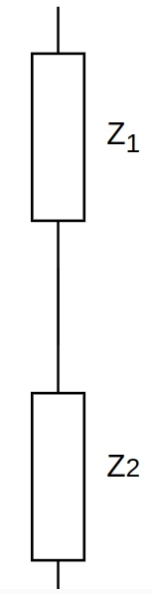
\includegraphics[height=6cm]{figures/ch00/series.jpg}
	\captionof{figure}{}
	\label{fig:series}
\end{minipage}
\begin{minipage}{.5\textwidth}
	\centering
	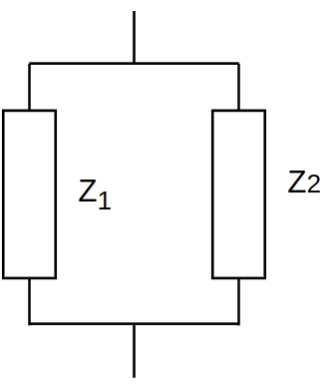
\includegraphics[width=4cm]{figures/ch00/parallel.jpg}
	\captionof{figure}{}
	\label{fig:parallel}
\end{minipage}%

Deux impédances sont en parallèle lorsqu'une même tension $V$ est appliquée à leurs bornes, comme illustré sur la figure \ref{fig:parallel}. Le courant à travers $Z_1$ est $V/Z_1$ et le courant à travers $Z_2$ est $V/Z_2$. Le courant total $I$ à travers les deux est donc $V/Z_1 + V/Z_2 = V \big(\frac{1}{Z_1} + \frac{1}{Z_2} \big) = \frac{V}{Z}$ avec $Z = \big(\frac{1}{Z_1} + \frac{1}{Z_2} \big)^{-1}$ la combinaison en parallèle de $Z_1$ et $Z_2$.

\subsection{Théorème de Millman}
Le théorème de Millman est dérivé de la loi de Kirchhoff sur les courants et permet de calculer la tension dans un nœud en fonction des tensions dans les nœuds voisins (voir figure \ref{fig:millman}):
\begin{equation}
	v_0 = \frac{\sum_{i=1}^n Y_i v_i + I_{eq}}{\sum_{i=1}^n Y_i}
	\label{eq:millman}
\end{equation}
avec $Y_i$ la conductance de chaque élément.
\begin{figure}[h!]
	\centering
	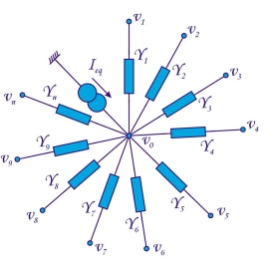
\includegraphics[width=6cm]{figures/ch00/millman.jpg}
	\caption{}
	\label{fig:millman}
\end{figure}
\\On peut déduire ce théorème en appliquant la loi de KCL au noeud $0$:
\begin{align*}
	\sum_{i = 1}^n I_n = \sum_{i = 1}^n Y_i(v_i - v_0) + I_{eq} = 0 \\
	\Rightarrow v_0 \; \sum_{i = 1}^n Y_i = \sum_{i = 1}^n Y_i\;v_i  + I_{eq} \\
	\Rightarrow v_0  = \frac{\sum_{i=1}^n Y_i v_i + I_{eq}}{\sum_{i=1}^n Y_i} 
\end{align*}
La tension dans le noeud $0$ est donc la moyenne pondérée des tensions environnantes, avec les conductances comme poids.

\subsection{Diagramme de Bode}
Appliquons les concepts de cette section au problème de la figure \ref{fig:example1}. Comme nous avons supposé que tous les signaux sont sinusoïdaux, nous posons que $v_{in} = V_0 e^{j\omega t}$. Par conséquent:
\begin{align*}
	V_{in} &= I \cdot R + \frac{1}{j \omega C} I \\
	\Rightarrow I &= \frac{j \omega C}{1 + j \omega RC} ; V_{in}\\
	\text{et} \quad V_C &= \frac{1}{1 + j \omega RC} ; V_{in}
\end{align*}
Nous pouvons donc conclure que:
\begin{align*}
	\frac{V_C}{V_{in}} &= \frac{1}{1 + j \omega RC} \\
	&= \frac{1}{\sqrt{1 + \omega^2 T^2}} e^{-j \phi}
\end{align*}
avec $\phi = \text{atan}(\omega ; T)$. Notez que nous ne trouvons aucune information sur la réponse transitoire comme précédemment, mais nous trouvons comment le circuit se comporte en \emph{régime harmonique permanent} (RHP).\
Le rapport $\frac{V_C}{V_{in}}$ est appelé \emph{transmittance} $H(\omega)$ et il a une amplitude $A = |T(\omega)|$ et une phase $\phi$. Lorsque nous traçons $20 \log(A)$ [dB] en fonction de $\log(\omega)$, nous trouvons la courbe de Bode:

$$
20 \log(A) = -20 \; \frac{1}{2} \; \log_{10}(1 + \omega^2 T^2)
$$
À partir de cette expression, nous déduisons que:
\begin{itemize}
	\item Lorsque $\omega T \ll 1$, $20 \log_{10}(A) \approx 20 \log_{10}(1) = 0$.
	\item D'autre part, lorsque $\omega T \gg 1$, $20 \log_{10}(A) \approx -20 \log_{10}(\omega T)$ et $|H(\omega)|$ diminue de $20$ dB pour chaque augmentation de $\omega$ d'un facteur de $10$ ($-20$ dB par décade).
\end{itemize}

En règle générale, toute transmittance $T(\omega)$ peut être écrite sous la forme :
$$
T(\omega) = A_0 \frac{(1 + j \omega T_{n+1}) \ldots (1 + j \omega T_{p})}{(1 + j \omega T_{1}) \ldots (1 + j \omega T_{n})}
$$
Chaque terme individuel est égal à $1$ si $\omega \ll 1/T_i$ ou égal à $j \omega T_i$ si $\omega \gg 1/T_i$. Par conséquent, une courbe de Bode peut être construite approximativement en suivant quelques règles simples : lorsque l'on rencontre une pulsation critique $\omega = 1/T$ dans le numérateur (un \emph{zéro}) ou dans le dénominateur (un \emph{pôle}), la courbe va :
\begin{itemize}
	\item décroître de $20$ dB par décade pour un pôle,
	\item augmenter de $20$ dB par décade pour un zéro,
\end{itemize}
Des règles similaires existent pour la phase $\phi$ du signal : chaque pôle introduit un décalage de $-\frac{\pi}{2}$, chaque zéro crée un décalage de $+\frac{\pi}{2}$. Notez que ces règles ne produisent qu'une estimation des courbes de Bode ; le tracé réel présentera un comportement plus compliqué, surtout lorsque les pôles sont complexes.\
Un exemple basé sur la figure \ref{fig:example1} est donné dans la figure \ref{fig:bode1}. Pour un système du premier ordre comme celui-ci, la coupure à -$3$ dB est atteinte à $\omega = \omega_0$, la pulsation critique.
\begin{figure}[h!]
	\centering
	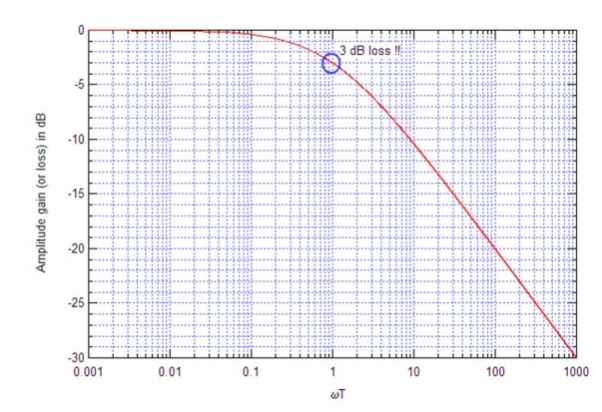
\includegraphics[width=10cm]{figures/ch00/bode.jpg}
	\caption{}
	\label{fig:bode1}
\end{figure}

\section{Transformations de circuits}
\subsection{Théorème de Thévenin}
Le théorème de Thévenin stipule qu'un réseau électrique linéaire à deux bornes peut être remplacé aux bornes A-B par une combinaison équivalente d'une source de tension $E_{Th}$ en série avec une impédance $Z_{Th}$. Deux circuits sont équivalents s'ils ont la même relation tension-courant à leurs bornes. Cette idée est illustrée dans la figure \ref{fig:thevenin}, où les éléments du circuit dans le nuage bleu sont remplacés par la source et l'impédance à droite.

\begin{itemize}
	\item La tension équivalente $E_{Th}$ est la tension obtenue aux bornes A-B du réseau avec les bornes A-B en circuit ouvert.
	\item L'impédance équivalente $Z_{Th}$ est l'impédance que le circuit entre les bornes A et B aurait si toutes les sources de tension idéales du circuit étaient remplacées par un court-circuit et toutes les sources de courant idéales étaient remplacées par un circuit ouvert.
\end{itemize}

\begin{minipage}{.5\textwidth}
	\centering
	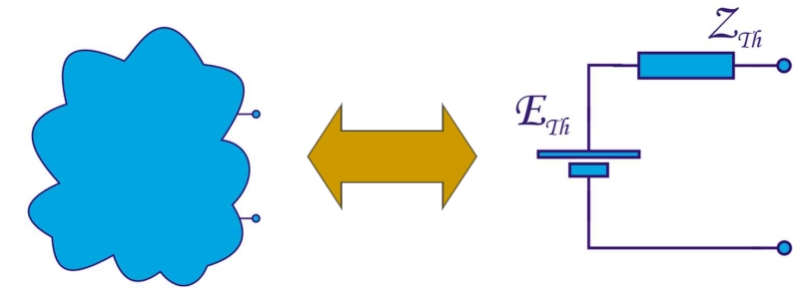
\includegraphics[width=7cm]{figures/ch00/thevenin.jpg}
	\captionof{figure}{Thévenin equivalent}
	\label{fig:thevenin}
\end{minipage}
\begin{minipage}{.5\textwidth}
	\centering
	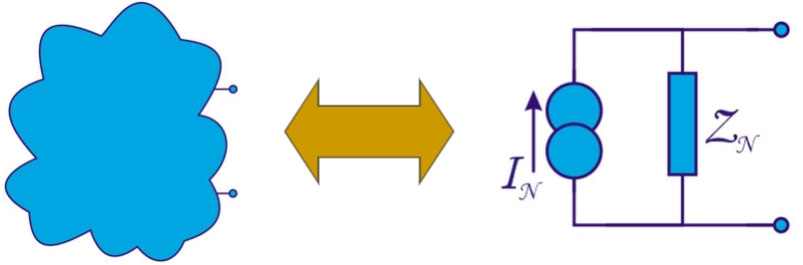
\includegraphics[width=7cm]{figures/ch00/norton.jpg}
	\captionof{figure}{Norton equivalent}
	\label{fig:norton}
\end{minipage}%

\subsection{Le théorème de Norton}
Le théorème de Norton nous indique comment remplacer un réseau linéaire par une source de courant $I_N$ en parallèle avec une impédance $Z_N$, comme illustré dans la figure \ref{fig:norton}. C'est le dual du théorème de Thévenin.
\begin{itemize}
	\item Le courant de Norton $I_N$ est calculé comme le courant qui circule aux bornes d'un court-circuit (résistance nulle entre les bornes de sortie).
	\item L'impédance $Z_N$ est trouvée en calculant la tension de sortie produite sans résistance connectée aux bornes; de manière équivalente, c'est la résistance entre les bornes avec toutes les sources de tension (indépendantes) court-circuitées et toutes les sources de courant (indépendantes) circuit ouvert. Cela équivaut à calculer la résistance de Thévenin : $Z_{Th} = Z_{N}$.
\end{itemize}
De plus, la tension de sortie générée par la source de Norton avec les bornes de sortie ouvertes est égale à la tension de Thévenin : $E_{Th} = Z_{N} ; I_N$.

\subsection{Deux Ports}
Certains circuits ont deux noeuds d'accès: une entrée et une sortie. Nous supposons que le port est unilatéral: les signaux transitent de l'entrée à la sortie et ne reviennent pas. Nous modélisons l'entrée comme une impédance $Z_i$ et la sortie comme un circuit équivalent Thévenin ou Norton - voir la figure \ref{fig:two_port}. Notez comment les sources de courant et de tension dépendent toutes deux de la tension d'entrée.
\begin{figure}[h!]
	\centering
	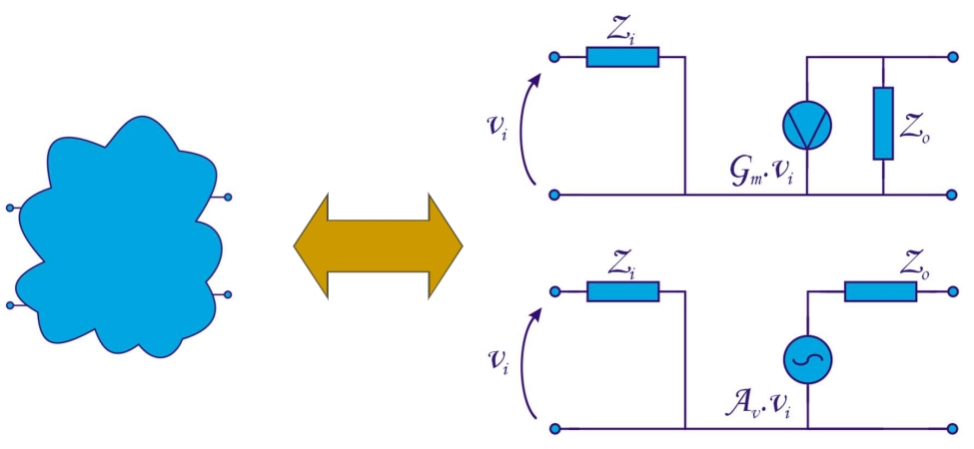
\includegraphics[width=12cm]{figures/ch00/two_port.jpg}
	\caption{}
	\label{fig:two_port}
\end{figure}
Les différents éléments ont des noms:
\begin{itemize}
	\item $Z_i$: l'impédance d'entrée,
	\item $Z_o$: l'impédance de sortie,
	\item $G_m$: la transconductance,
	\item $A_v$: le gain de tension.
\end{itemize}
Ils peuvent être calculés de la manière suivante:
\begin{itemize}
	\item $Z_i$: appliquer une tension d'entrée $V_i$, calculer le courant d'entrée $I_i$. Ensuite, $Z_i = \frac{V_i}{I_i}$;
	\item $Z_o$: éliminer la transconductance en reliant l'entrée à la masse: $V_i = 0$, appliquer une tension $V_o$ à la sortie et calculer le courant de sortie $I_o$. Ensuite, $Z_o = \frac{V_o}{I_o}$.
	\item $G_m$: court-circuiter la sortie de sorte qu'aucun courant ne passe à travers $Z_o$. Appliquer une tension d'entrée $V_i$ et calculer le courant de sortie $I_o$. Ensuite, $G_m = \frac{I_o}{V_i}$.
	\item $A_v$: garder la sortie ouverte. Appliquer une tension d'entrée $V_i$ et calculer la tension de sortie $V_o$. Ensuite, $A_v = \frac{V_o}{V_i}$.
\end{itemize}


\subsection{Circuits en cascade}

Lorsque plusieurs circuits sont connectés en cascade, on parle de circuits en cascade. Ils se composent généralement de :

\begin{itemize}
	\item Une source, telle qu'une antenne, un générateur de signal ou un microphone, que l'on modélise comme une source de courant $i_s$ ou de tension $v_s$, en parallèle ou en série avec une impédance de sortie $Z_s$.
	\item Un étage intermédiaire tel qu'un amplificateur ou un filtre qui transforme réellement le signal. Cet étage a une impédance d'entrée $Z_i$, une impédance de sortie $Z_o$, un gain de tension $A_v$ ou une transconductance $G_m$.
	\item Une charge, qui peut être un PC, un oscilloscope, un haut-parleur, ... Nous modélisons cela comme une impédance de charge $Z_l$.
\end{itemize}

Cette configuration est illustrée dans la figure \ref{fig:cascade}.

Si nous ne faisons pas attention, chaque étage influencera l'étage précédent ou suivant. Nous pouvons calculer la relation entre le courant de source $i_s$ et la tension de charge $v_l$ dans la figure \ref{fig:cascade} :

\begin{itemize}
	\item La tension $v_i$ aux bornes de $Z_i$ est :
	$$v_i = i_s\;(Z_s || Z_i) = \frac{Z_s Z_i}{Zs+Z_i} i_i$$
	et pas simplement $i_s;Z_s$. L'étage intermédiaire charge l'étage source.
	\item La tension de charge $v_l$ aux bornes de $Z_l$ est :
	$$v_l = - G_m (Z_o || Z_l) v_i = -G_m \frac{Z_o Z_l}{Z_o + Z_l} v_i$$ 
	et pas simplement $-G_m Z_l v_i$. L'impédance de sortie de l'étage intermédiaire s'ajoute à la charge.
	\item Cela signifie que la tension du signal disponible en sortie est :
	$$v_l = -G_m Z_o  \frac{Z_l}{Z_o + Z_l} \frac{Z_i}{Zs+Z_i} Z_s i_i = \frac{Z_l}{Z_o + Z_l} \frac{Z_i}{Zs+Z_i} A_v v_s$$
\end{itemize}
Idéalement, cela devrait être $v_l = - A_v v_s$. À partir de cela, nous pouvons conclure que $Z_i \rightarrow \infty$ et que $Z_o \rightarrow 0$ pour se rapprocher du comportement idéal. Nous devons concevoir pour avoir une impédance d'entrée élevée et une impédance de sortie faible.